\section{Relasjonsalgebra}
\subsection*{Operatorer}
\begin{frame}{Operatorer}
\begin{tabular}{l|l|l}
 Operator & Betydning & Eksempel\\\hline
 $\pi_{columns}(Tabell)$ & Projection (SELECT DISTINCT) & $\pi_{title, year}(Film)$\\\pause
 $\sigma_{condition}(Tabell)$ & Condition (WHERE) & $\sigma_{year > 2015}(Film)$\\\pause
 $A \times B$ & Cross join / Cartesian product & $Film \times Screening$\\\pause
 $A \cap B$ & Intersection & $Film1 \cap Film2$ \\\pause
 $A \cup B$ & Union & $Film1 \cup Film2$ \\\pause
 $A \setminus B$ & Set difference &  $Film1 \setminus Film2$\\\pause
 $A \bowtie_{condition} B$ & Inner Join & $A \bowtie_{{film\_id}={film\_id}} B$
\end{tabular}
\end{frame}

\subsection*{Eksempler}
\begin{frame}[fragile]{Eksempel 1}
\begin{minted}{sql}
SELECT DISTINCT Country
FROM Film
WHERE year < 1950
\end{minted}
\pause
$\pi_{Country}\textcolor{blue}{(}\sigma_{year < 1950}\textcolor{red}{(}Film\textcolor{red}{)}\textcolor{blue}{)}$
\end{frame}

\begin{frame}[fragile]{Eksempel 2}
\begin{minted}{sql}
SELECT DISTINCT title, year
FROM Film, Director
WHERE Film.dir_id = Director.id
AND Film.year = 1992
\end{minted}
\pause
$\pi_{title, year}\textcolor{blue}{(}\sigma_{year = 1992}\textcolor{red}{(}Film\textcolor{red}{)} \bowtie_{Film.dir\_id=Director.id}\textcolor{red}{(}Director\textcolor{red}{)}\textcolor{blue}{)}$
\end{frame}

\begin{frame}[fragile]{Eksempel 3}
\begin{minted}{sql}
SELECT Country.name, capital, inhabitants
FROM Country, City
WHERE Country.capital = City.id
AND inhabitants < 500000
\end{minted}
\pause
$\pi_{Country.name, capital, inhabitants}\textcolor{blue}{(}\sigma_{inhabitants < 500000}\textcolor{green}{(}\textcolor{red}{(}Country\textcolor{red}{)}\bowtie_{Capital=City.id}\textcolor{red}{(}City\textcolor{red}{)}\textcolor{green}{)}\textcolor{blue}{)}$
\end{frame}

\subsection*{Spørretid}
\begin{frame}{Spørsmål?}
    \begin{figure}
        \centering
        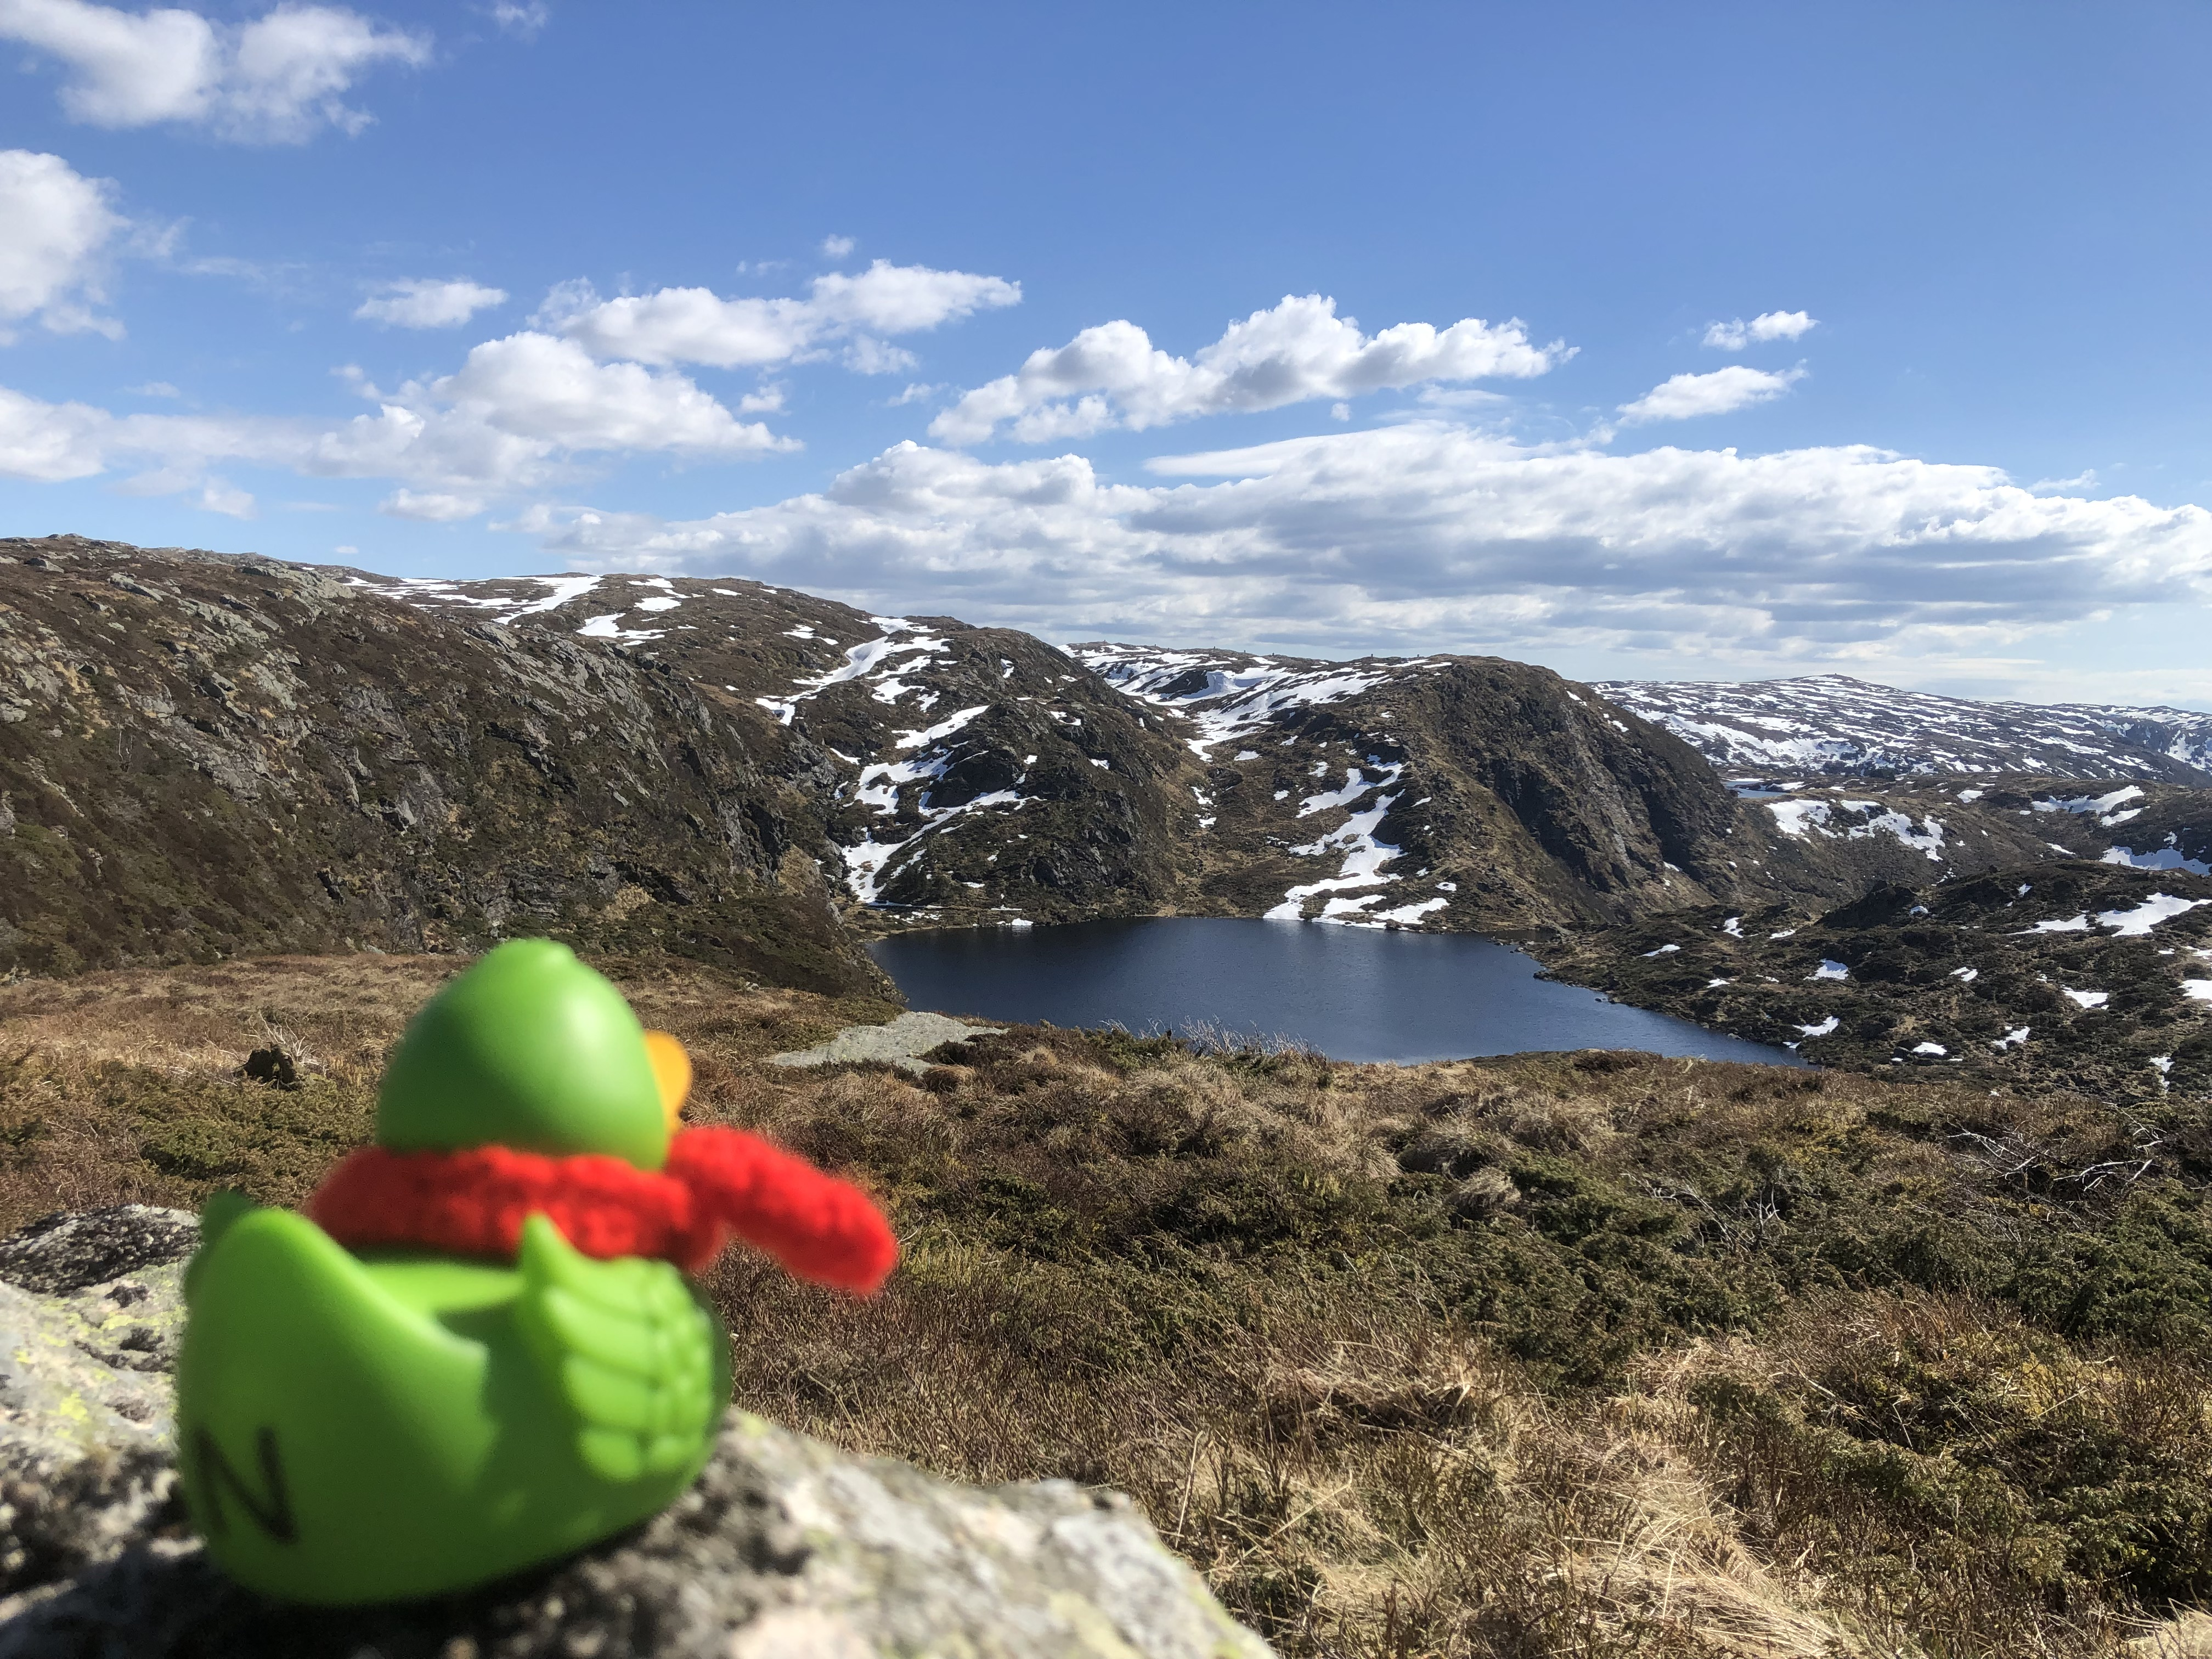
\includegraphics[height = 4.9cm]{images/guillaume4.jpg}
        \caption{Guillaume på Vidden}
        \label{fig:guillaume4}
    \end{figure}
\end{frame}